%!TEX root = main.tex
\section{Results and Discussion\label{sec:results}}

  \subsection{Experimental Setup}

  \subsection{Evaluation Metrics}
   \par  A sub-sampled dataset was created from the full dataset to determine the efficacy of these algorithms on varying number of worker responses, based on Table.\ref{batch_sample}. The number of workers plotted indicates the number of distinct worker segmentation used in the algorithm, note that in the clustered cases, the actual number of segmentation in the cluster may be less than what is cited in the sample. In the subsequent section, we will refer to objects specific to a sample synonymously as objects.
  \begin{table}[ht]
  \centering
  \label{batch_sample}
  \caption{Every object was randomly sampled worker with replacement. For small worker samples, we average our results over larger number of batches than for large worker samples (which have lower variance, since the sample size is close to the original data size).}
  \begin{tabular}{l|llllll}
  \# of workers & 5  & 10 & 15 & 20 & 25 & 30 \\ \hline
  \# of batches & 10 & 8  & 6  & 4  & 2  & 1 
  \end{tabular}
  \end{table}
   \par Evaluation metrics used in our experiment measures how well the final segmentation(S) produced by these algorithms compare against ground truth(GT). The most common evaluation metric used in literature are area-based methods which take into account the intersection, $\mathcal{I}=area(S\cup GT)$, or union, $\mathcal{U}=area(S\cap GT)$, between the user and the ground truth bounding boxes.
    $$\text{Precision (P)} = \frac{\mathcal{I}}{area(S)}$$ \\
    $$\text{Recall (R)} = \frac{\mathcal{I}}{area(GT)}$$ \\
    $$\text{Jaccard (J)} = \frac{\mathcal{U}}{\mathcal{I}}$$ \\
    $$\text{False Positive Rate (FPR)}= \frac{area(S)-\mathcal{I}}{area(GT)}$$\\
    $$\text{False Negative Rate (FNR)}= \frac{area(GT)-\mathcal{I}}{(area(S)-\mathcal{I})+(area(Image)-\mathcal{U})}$$
%%%%%%%%%%%%%%%%%%%%%%%%%%%%%%%%%%%%%%%%%%%%%%%%%%%%%%%%%%%%%%%%%%%%%%%%%%%%%%%%%%%%%%%%%%%%%%%%%%%%%%%%%%%%%%%%%%%%%%%%%%%%%%%%%%%%%%%%%%
  \subsection{What is the difference in performance between retrieval and aggregation-based methods?}
    As shown in Figure \ref{retreival_vs_aggregation}, we performed for the best performing ---- for each family of algo (including clustering)
    \begin{figure}[ht!]
      \centering
      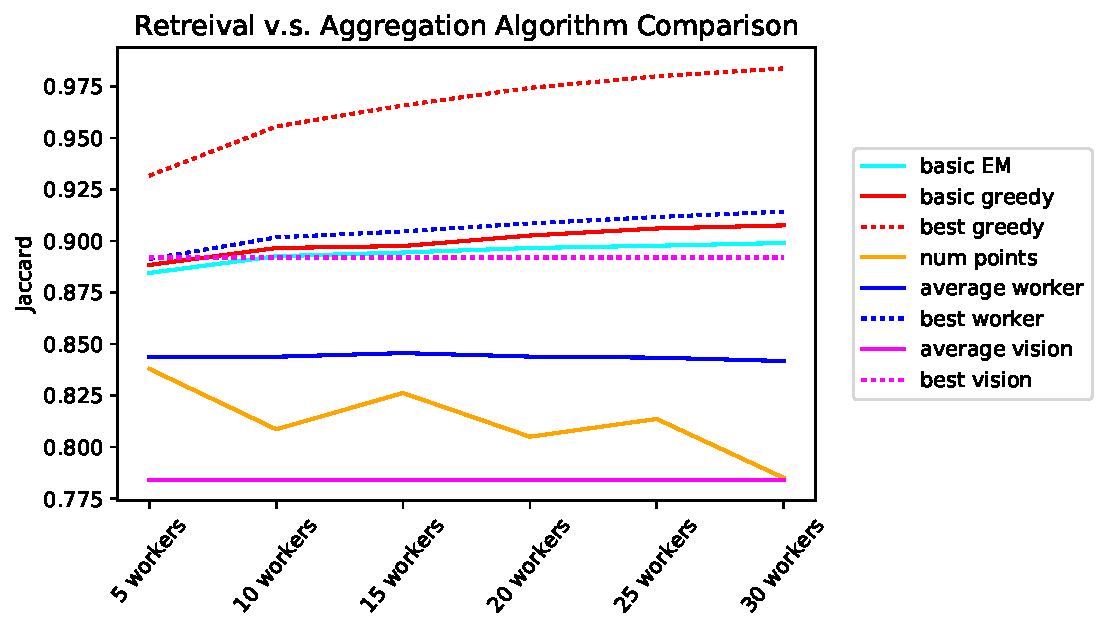
\includegraphics[width=\textwidth]{plots/Retreival_vs_Aggregation.pdf}
      \caption{Performance comparison between best-performing algorithms from retrieval and aggregation-based methods. Color denotes the type of algorithm used and dotted line shows the corresponding algorithm that makes use of ground truth.}
      \label{retreival_vs_aggregation}
    \end{figure}
      \ta{Key advantages of using aggregation-based approaches is due to its performance scalability as more annotations are collected as well as operating at a finer granularity that results in a higher potential upper bound.} Future work on developing better inference models would bring the performance closer to these upper bounds.
      
%%%%%%%%%%%%%%%%%%%%%%%%%%%%%%%%%%%%%%%%%%%%%%%%%%%%%%%%%%%%%%%%%%%%%%%%%%%%%%%%%%%%%%%%%%%%%%%%%%%%%%%%%%%%%%%%%%%%%%%%%%%%%%%%%%%%%%%%%%
  \subsection{How well does the inferred worker qualities predict individual worker performance?}
    \subsubsection{Correlation of worker qualities against performance}
     To further study whether the inferred worker qualities is indicative of the quality of an annotation, we independently performed linear fitting for each sample-objects and computed the $R^2$ statistics to determine whether worker qualities can predict precision, recall, and Jaccard. Table --- cites the ---- of the no clustering cases. Visual inspection of the basic worker quality model fitting showed that for objects that suffered from type two errors, the single-parameter worker quality could not predict the low precision that lead to a low Jaccard. The high correlation score implies that our advanced worker qualities are able to capture the 
    \subsubsection{EM performance with different worker quality models}


    \subsubsection{Best worker quality retrieval}
    One application of worker qualities is that it could be used as an annotation scoring function for retrieving the best quality worker segmentation. We explored this approach by training a linear regression model for every sample-object and use the worker qualities to predict the precision, recall, and Jaccard of individual worker annotations against ground truth. We query the model with the inferred worker quality and retrieve the worker with the best predicted Jaccard. 
    \par We chose to use a linear regression model rather than simply sorting the worker qualities and picking the best is that worker qualities in our advanced models are specifically designed to capture cases of false positives and false negatives that yields very different recall and precision values. Sorting based on multiple worker qualities effectively applies equal weighting to all quality attributes. We have tested that the linear regression model performs better on this task that simple sorting is capable of learning the weights that helps it make better predictions.
    \par 
%%%%%%%%%%%%%%%%%%%%%%%%%%%%%%%%%%%%%%%%%%%%%%%%%%%%%%%%%%%%%%%%%%%%%%%%%%%%%%%%%%%%%%%%%%%%%%%%%%%%%%%%%%%%%%%%%%%%%%%%%%%%%%%%%%%%%%%%%%
  \subsection{How do different families of aggregation based algorithms (EM v.s. Greedy v.s. MV) relate and compare?}
    Given the success of aggregation-based models, we wanted to further study how different algorithms perform compared to one another.

    
    \ta{We show that majority vote, while simple, performs nearly as well as the advanced EM and greedy based approaches.} This is because convergence.



    When using ground truth to estimate intersection areas, we can achieve a Jaccard of 0.983 as an upper bound with 30 workers, which indicates that with better probabilistic estimation of intersection area, aggregation-based methods can achieve close to perfect segmentation outputs, exceeding the results than that of any single `best' worker (J= --- for 30 workers). Suggest precise BB useful for some application.
%%%%%%%%%%%%%%%%%%%%%%%%%%%%%%%%%%%%%%%%%%%%%%%%%%%%%%%%%%%%%%%%%%%%%%%%%%%%%%%%%%%%%%%%%%%%%%%%%%%%%%%%%%%%%%%%%%%%%%%%%%%%%%%%%%%%%%%%%%
  \subsection{How well does clustering resolve multiple perspectives of crowdworkers and improve quality evaluation algorithms?}
    \begin{figure}[ht!]
      \centering
      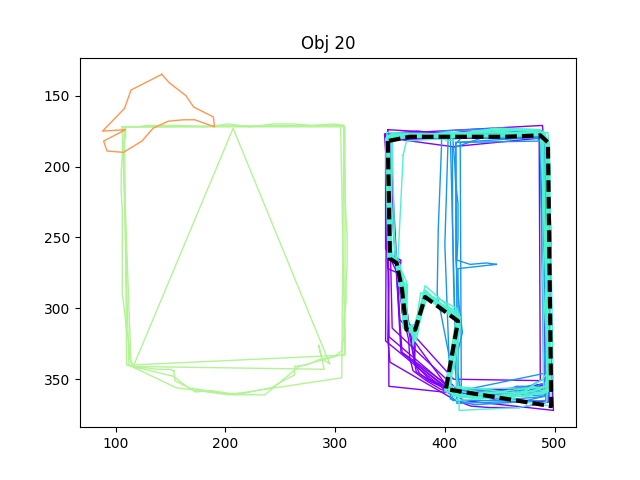
\includegraphics[width=\textwidth]{plots/20.png}
      \caption{TODO}
      \label{cluster_example}
    \end{figure}
    \begin{figure}[ht!]
      \centering
      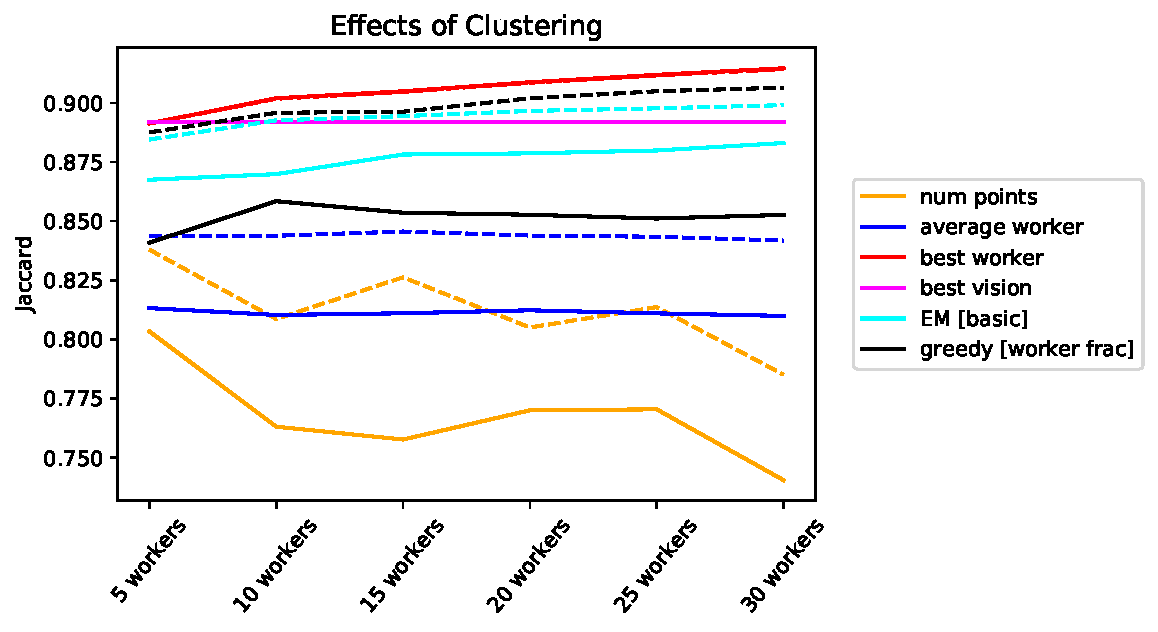
\includegraphics[width=\textwidth]{plots/Effects_of_clustering.pdf}
      \caption{TODO}
      \label{cluster_effect}
    \end{figure}
  \par Compared to using a metric-based heuristic to detect and eliminate these errors, clustering has additional benefit of preserving worker's semantic intentions in the case where there are multiple instances of different errors. For example, in the object 20 example above, the mistakened clusters included semantic concepts ``monitor'', ``computer'', ``turtle'', ``computer front''. While these are considered bad annotations for this particular task, this cluster of annotation can provide more data for another semantic task ``monitor''. A potential direction of future work includes adding a additional crowdsourcing task for semantic labelling of clusters (which is cheaper and more accurate than segmentation) to enable reuse of annotations across objects and lowering the cost of data collection. 


%%%%%%%%%%%%%%%%%%%%%%%%%%%%%%%%%%%%%%%%%%%%%%%%%%%%%%%%%%%%%%%%%%%%%%%%%%%%%%%%%%%%%%%%%%%%%%%%%%%%%%%%%%%%%%%%%%%%%%%%%%%%%%%%%%%%%%%%%%
  \subsection{Can vision information be used to improve the crowdsourced responses?}
  We explored the idea of using a vision algorithm to improve aggregation-based quality evaluation methods. 